% \documentclass[../main.tex]{subfiles}

% \begin{document}

{
\setstretch{1.0}
\chapter*{Supplementary figures}
\addcontentsline{toc}{chapter}{Supplementary figures}
\label{supp_fig}
\markboth{Supplementary figures}{Supplementary figures}
}

High-quality supplementary figures are available at the following GitHub repository:

\underline{\href{https://github.com/filonico/phd_thesis_tex}{https://github.com/filonico/phd\_thesis\_tex}}

\setcounter{figure}{0}
\renewcommand{\figurename}{Supplementary Figure}
\renewcommand{\thefigure}{\textbf{S\arabic{figure}}}

\begin{figure}[ht]
	\centering
	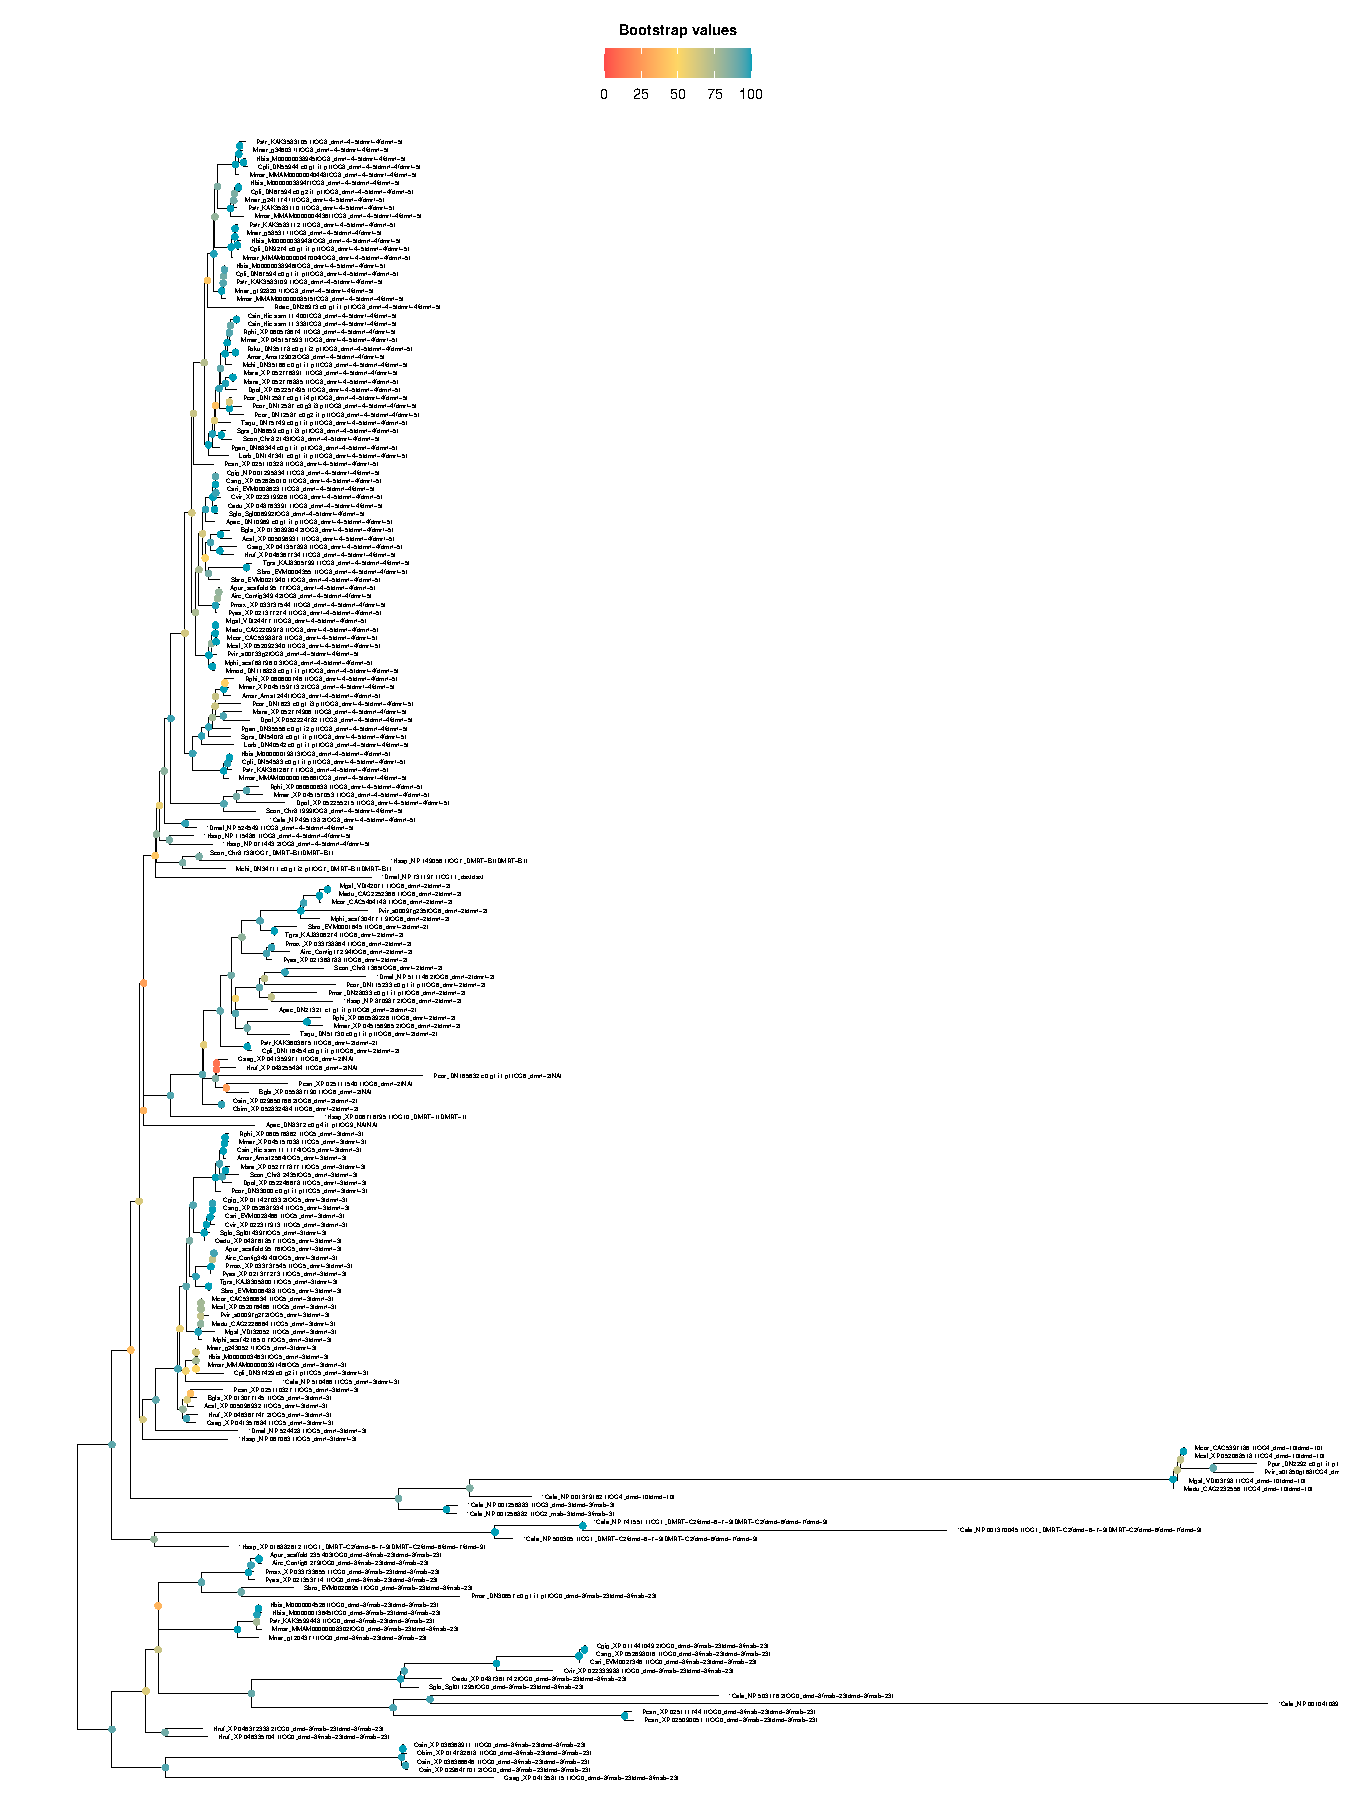
\includegraphics[width=0.7\textwidth]{supp_figures/supp_fig_S1.pdf}
	\caption[\textbf{\gls{ml} phylogenetic tree of the Dmrt gene family in molluscs, including the possvm orthology inference}]
	{
		\textbf{\gls{ml} phylogenetic tree of the Dmrt gene family in molluscs, including the possvm orthology inference}. Reference genes from \gls{hsap}, \gls{cele}, and \gls{dmel} are marked with an asterisk at the beginning of the tip names. Species ID can be found in \cref{suppTab:bivalve_dataset}. The tree has been midpoint rooted. Bootstrap values are shown for each node.
	}
	\label{suppFig:dmrt_bivalves}
\end{figure}

\begin{figure}[ht]
	\centering
	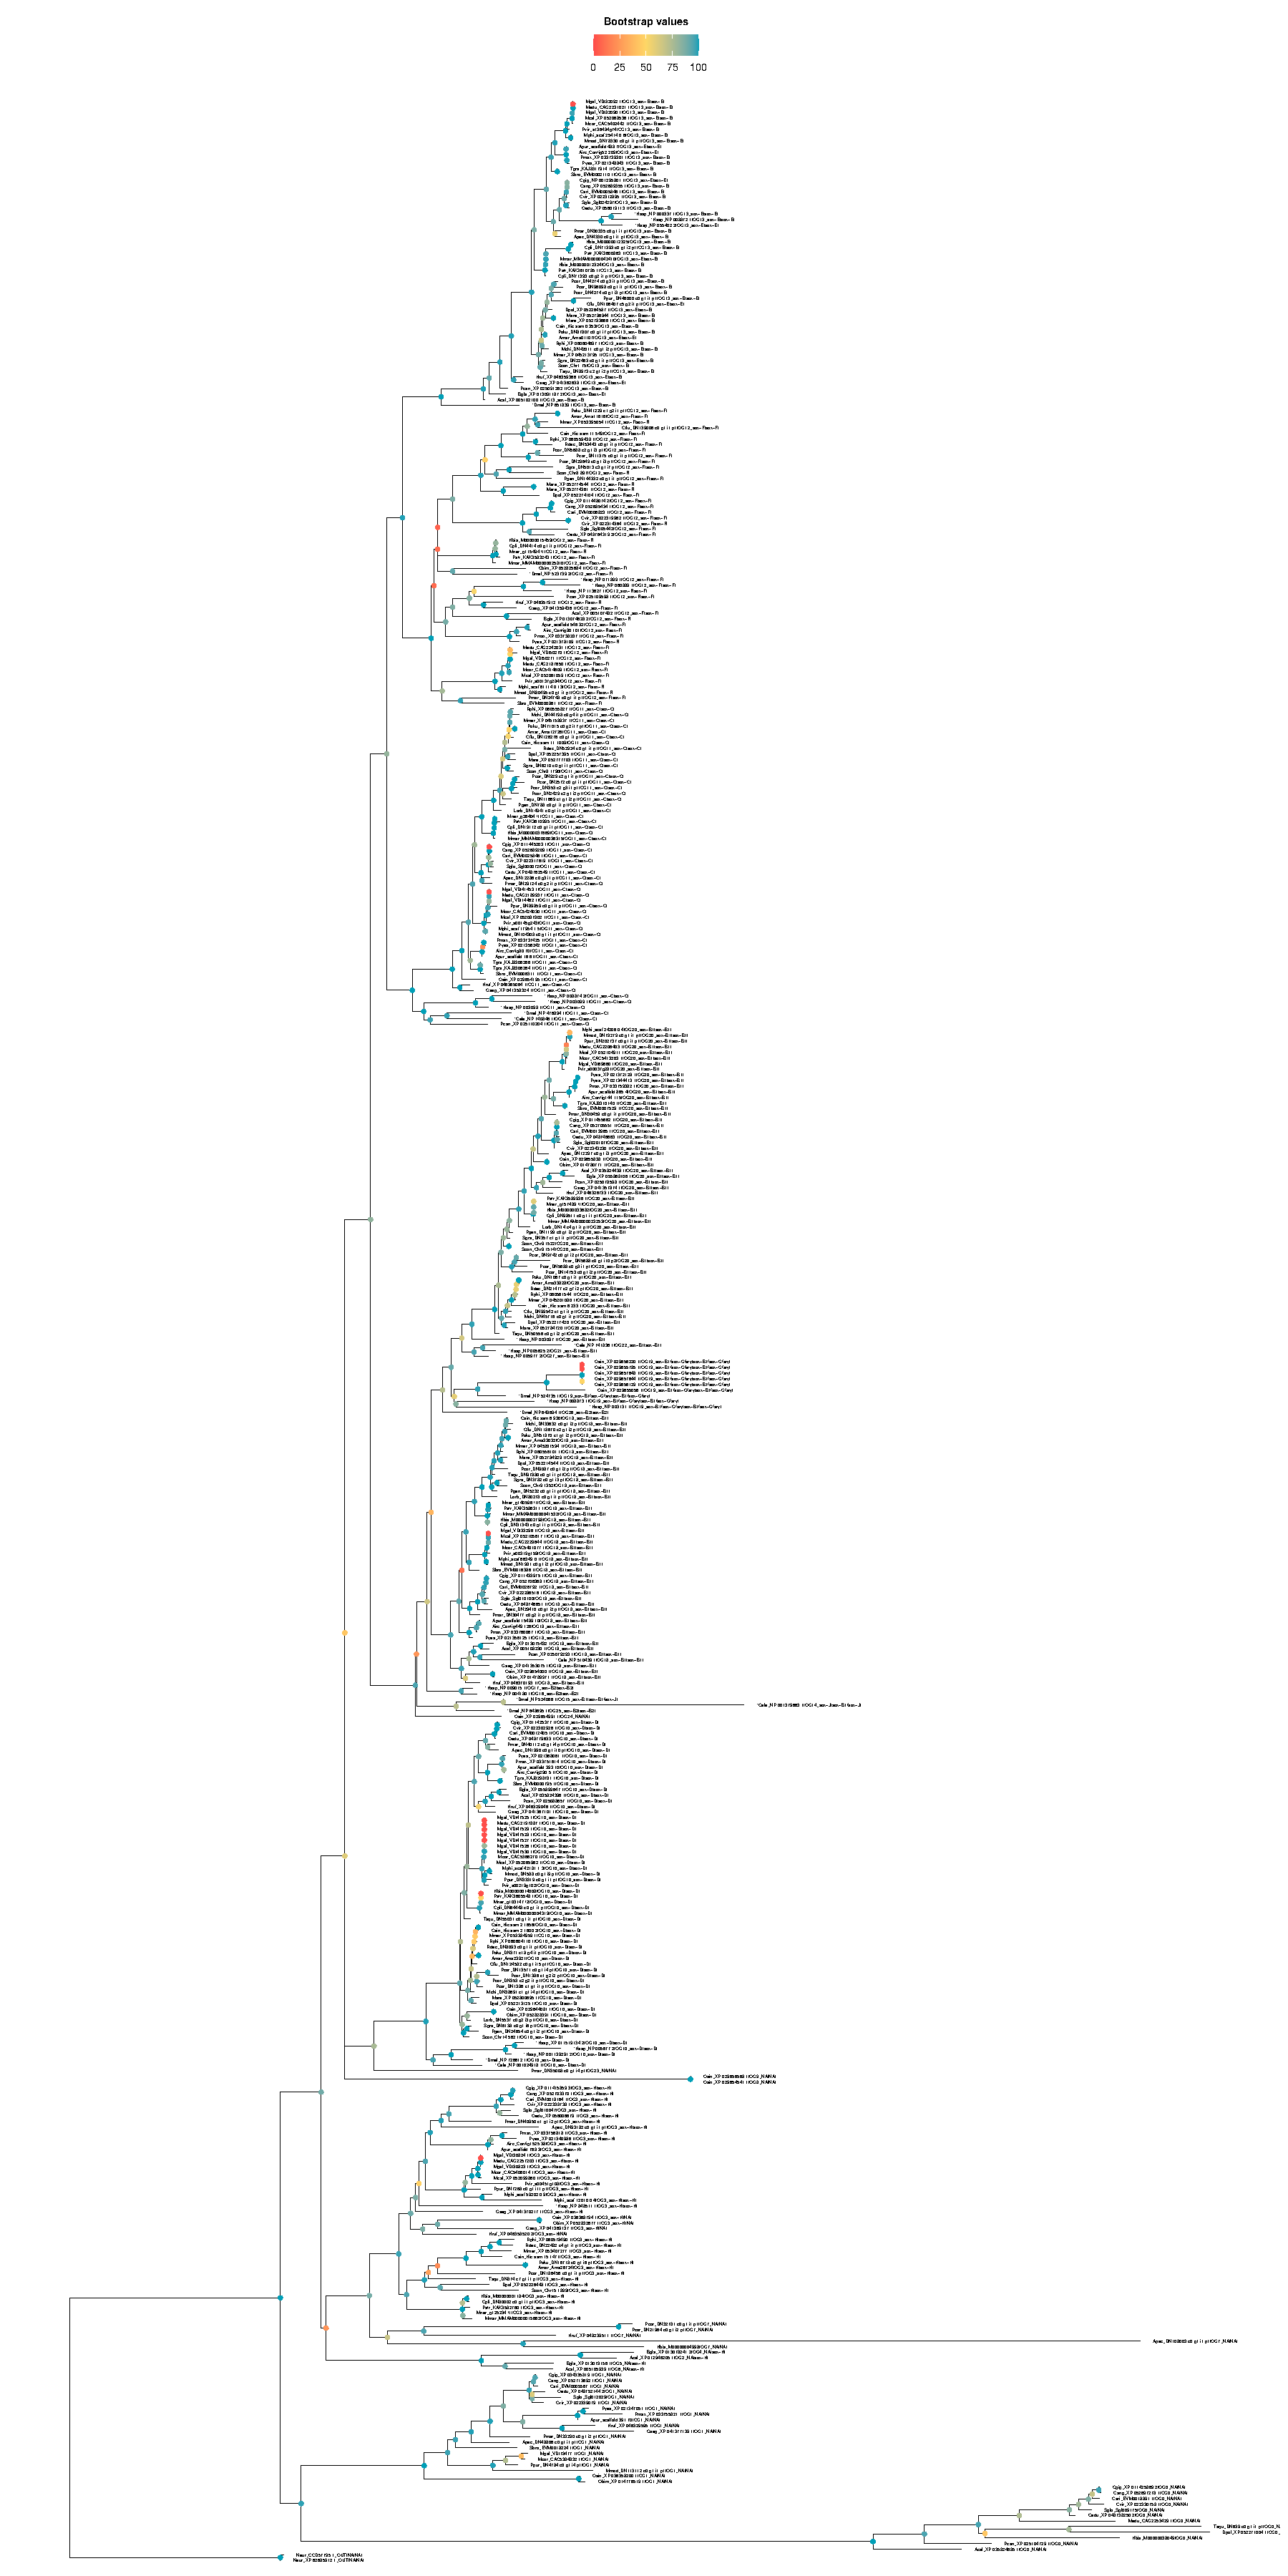
\includegraphics[height=0.9\textheight]{supp_figures/supp_fig_S2.pdf}
	\caption[\textbf{\gls{ml} phylogenetic tree of the Sox gene family in molluscs, including the possvm orthology inference}]
	{
		\textbf{\gls{ml} phylogenetic tree of the Sox gene family in molluscs, including the possvm orthology inference}. Reference genes from \gls{hsap}, \gls{cele}, and \gls{dmel} are marked with an asterisk at the beginning of the tip names. Species ID can be found in \cref{suppTab:bivalve_dataset}. Bootstrap values are shown for each node.
	}
	\label{suppFig:sox_bivalves}
\end{figure}

\begin{figure}[ht]
	\centering
	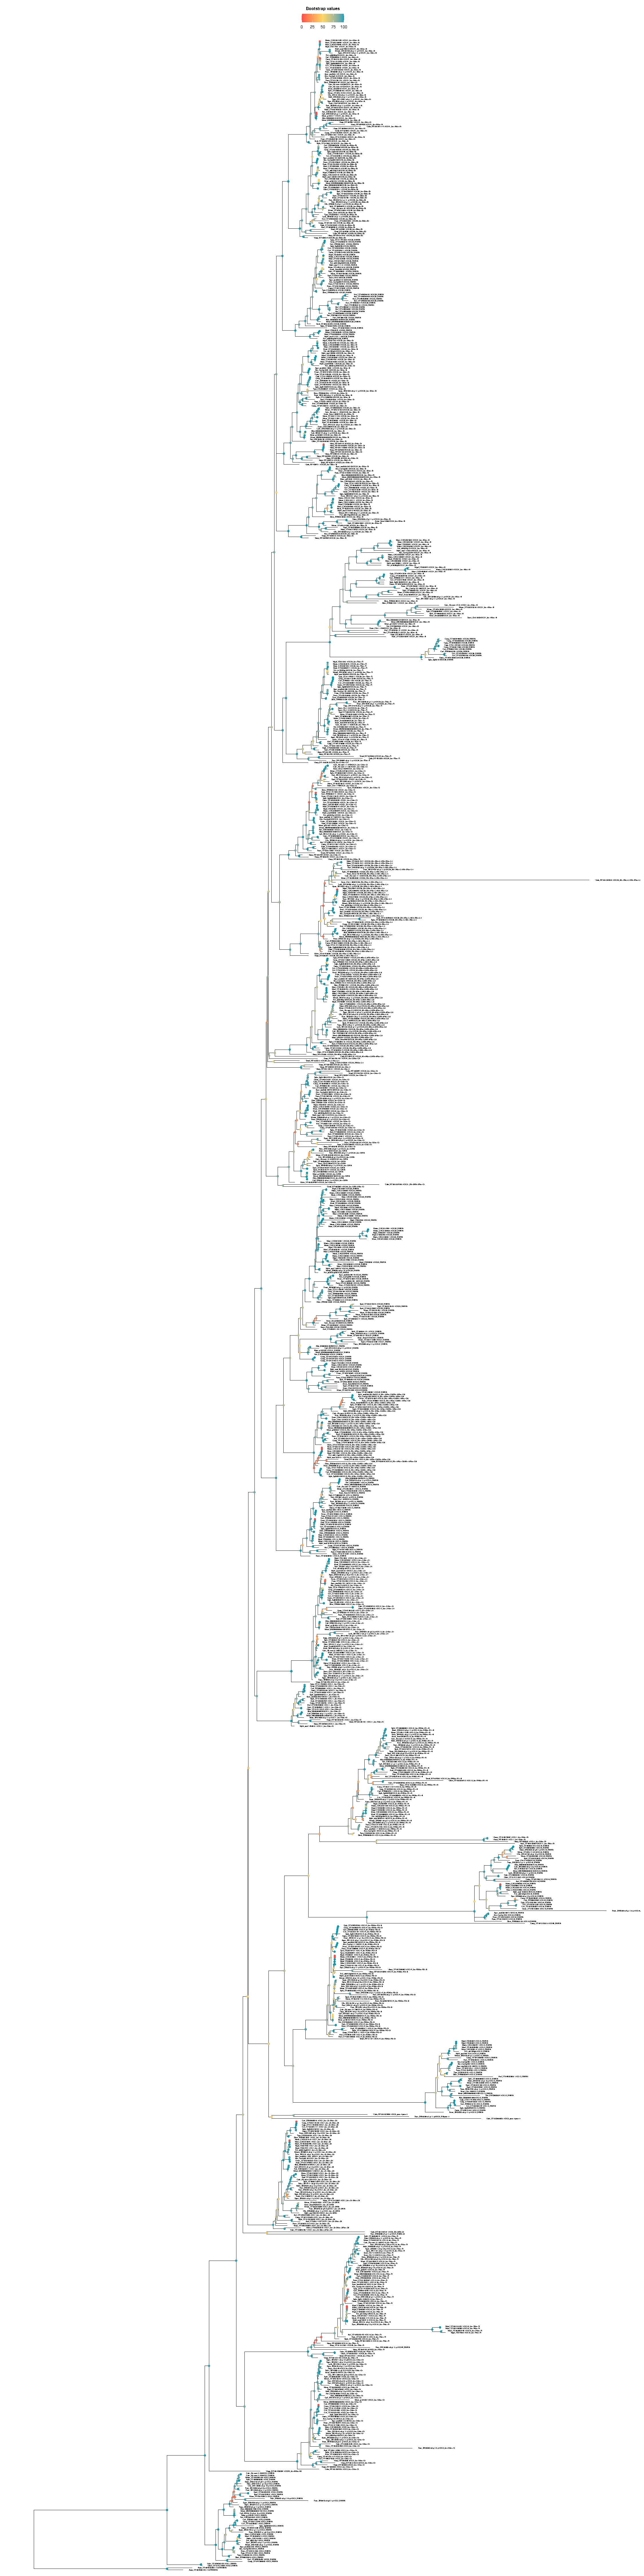
\includegraphics[height=0.9\textheight]{supp_figures/supp_fig_S3.pdf}
	\caption[\textbf{\gls{ml} phylogenetic tree of the Fox gene family in molluscs, including the possvm orthology inference}]
	{
		\textbf{\gls{ml} phylogenetic tree of the Fox gene family in molluscs, including the possvm orthology inference}. Reference genes from \gls{hsap}, \gls{cele}, and \gls{dmel} are marked with an asterisk at the beginning of the tip names. Species ID can be found in \cref{suppTab:bivalve_dataset}. Bootstrap values are shown for each node.
	}
	\label{suppFig:fox_bivalves}
\end{figure}

\begin{figure}[ht]
	\centering
	\includegraphics[width=0.95\textwidth]{supp_figures/supp_fig_S4.png}
	\captionsetup[subfigure]{labelformat=nocaption}
	\begin{subfigure}{0\linewidth}
	\caption{}\label{suppFig:DSFG_testCompilation-A}
	\end{subfigure}% <----- get rid of space, for proper centering
	\begin{subfigure}{0\linewidth}
	\caption{}\label{suppFig:DSFG_testCompilation-B}
	\end{subfigure}% <----- get rid of space, for proper centering
	\caption[\textbf{The DSFG complement in Mammalia and \textit{Drosophila} spp.}]
	{
		\textbf{The DSFG complement in Mammalia (A) and \textit{Drosophila} spp. (B)}. Presence/absence of genes in various species are indicated by filled circles. Numbers inside each circle specify genes with 2 or more copies. The shaded area highlights outgroup species, \gls{ggal} (Aves) for mammals and \gls{agam} (Culicidae) for fruit flies. The phylogenetic tree of analysed species, as inferred from literature, is shown on the left, while major taxonomic groups are reported on the right. All species are represented by genomic data. \gls{dsfg} trees are shown on the bottom (full trees can be found in \cref{suppFig:dmrt_mammals,suppFig:fox_mammals}). Full species names for both mammals and fruit flies, along with all assembly and taxonomic information, can be found in \cref{suppTab:mammal_dataset,suppTab:drosophila_dataset}, respectively. A.: Aves; Chirop.: Chiroptera; L.: Lagomorpha; M.: Monotremata; Me.: Metatheria; P.: Pholidota; Pe.: Perissodactyla; Prim.: Primates; Roden.: Rodentia; X.: Xenarthra; C.: Culicidae.
	}
	\label{suppFig:DSFG_testCompilation}
\end{figure}

\begin{figure}[ht]
	\centering
	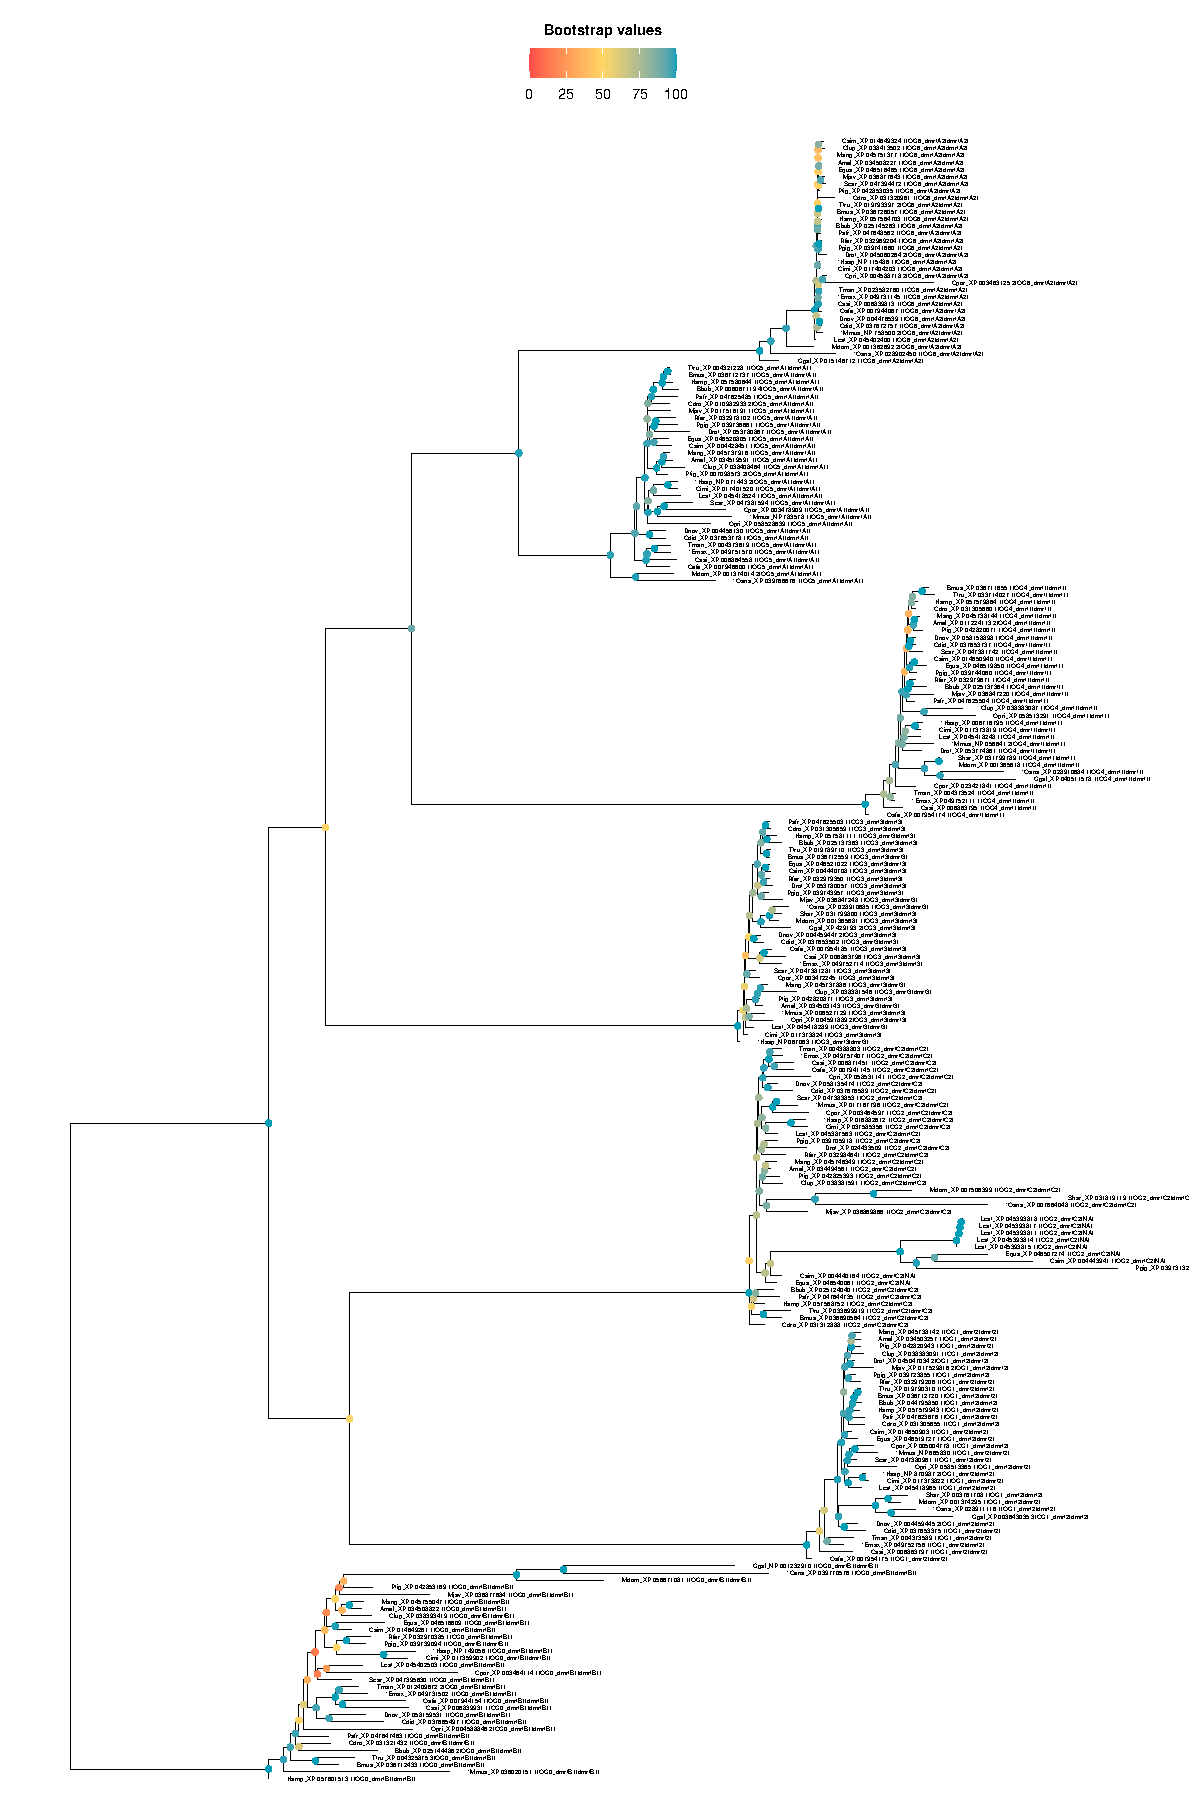
\includegraphics[height=0.85\textheight]{supp_figures/supp_fig_S5.pdf}
	\caption[\textbf{\gls{ml} phylogenetic tree of the \gls{dmrt} gene family in mammals, including the Possvm orthology inference}]
	{
		\textbf{\gls{ml} phylogenetic tree of the \gls{dmrt} gene family in mammals, including the Possvm orthology inference}. Reference genes from \gls{hsap}, \gls{mmus}, \gls{emax}, and \gls{oana} are marked with an asterisk at the beginning of the tip names. Species ID can be found in \cref{suppTab:mammal_dataset}. The tree has been midpoint rooted. Bootstrap values are shown for each node.
	}
	\label{suppFig:dmrt_mammals}
\end{figure}

\begin{figure}[ht]
	\centering
	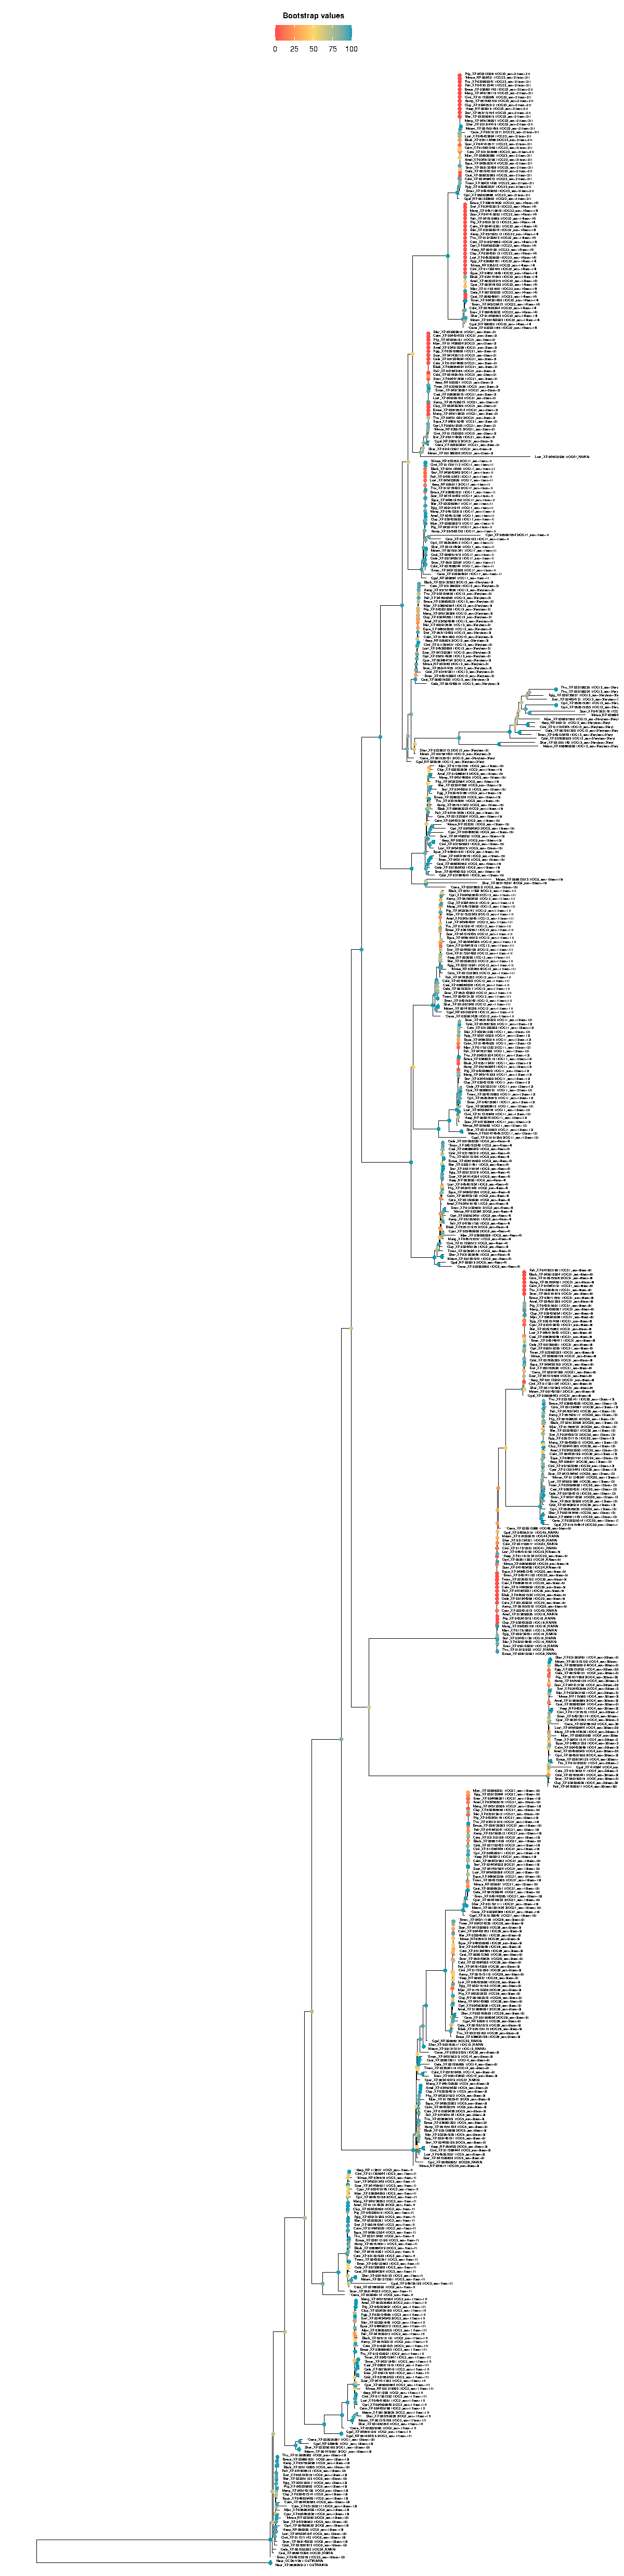
\includegraphics[height=0.85\textheight]{supp_figures/supp_fig_S6.pdf}
	\caption[\textbf{\gls{ml} phylogenetic tree of the \gls{sox} gene family in mammals, including the Possvm orthology inference}]
	{
		\textbf{\gls{ml} phylogenetic tree of the \gls{sox} gene family in mammals, including the Possvm orthology inference}. Reference genes from \gls{hsap}, \gls{mmus}, \gls{emax}, and \gls{oana} are marked with an asterisk at the beginning of the tip names. Species ID can be found in \cref{suppTab:mammal_dataset}. Bootstrap values are shown for each node.
	}
	\label{suppFig:sox_mammals}
\end{figure}

\begin{figure}[ht]
	\centering
	
\includegraphics[height=0.85\textheight]{supp_figures/supp_fig_S7.pdf}
	\caption[\textbf{\gls{ml} phylogenetic tree of the \gls{fox} gene family in mammals, including the Possvm orthology inference}]
	{
		\textbf{\gls{ml} phylogenetic tree of the \gls{fox} gene family in mammals, including the Possvm orthology inference}. Reference genes from \gls{hsap}, \gls{mmus}, \gls{emax}, and \gls{oana} are marked with an asterisk at the beginning of the tip names. Species ID can be found in \cref{suppTab:mammal_dataset}. Bootstrap values are shown for each node.
	}
	\label{suppFig:fox_mammals}
\end{figure}

\begin{figure}[ht]
	\centering
	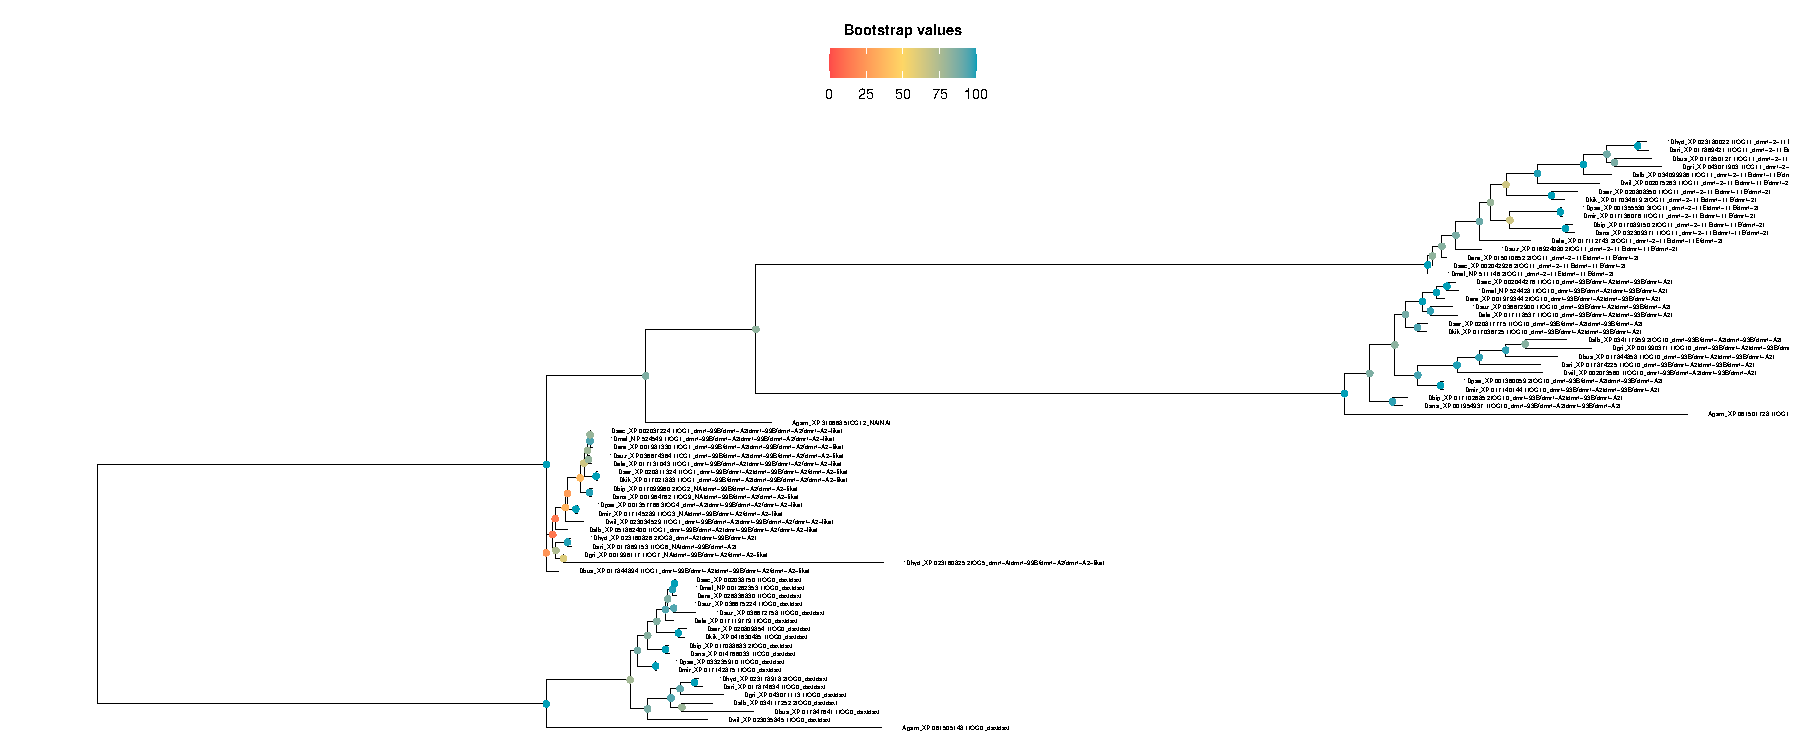
\includegraphics[width=\textwidth]{supp_figures/supp_fig_S8.pdf}
	\caption[\textbf{\gls{ml} phylogenetic tree of the \gls{dmrt} gene family in fruit flies, including the Possvm orthology inference}]
	{
		\textbf{\gls{ml} phylogenetic tree of the \gls{dmrt} gene family in fruit flies, including the Possvm orthology inference}. Reference genes from \gls{dmel}, \gls{dhyd}, \gls{dpse}, and \gls{dsuz} are marked with an asterisk at the beginning of the tip names. Species ID can be found in \cref{suppTab:drosophila_dataset}. The tree has been midpoint rooted. Bootstrap values are shown for each node.
	}
	\label{suppFig:dmrt_drosophila}
\end{figure}

\begin{figure}[ht]
	\centering
	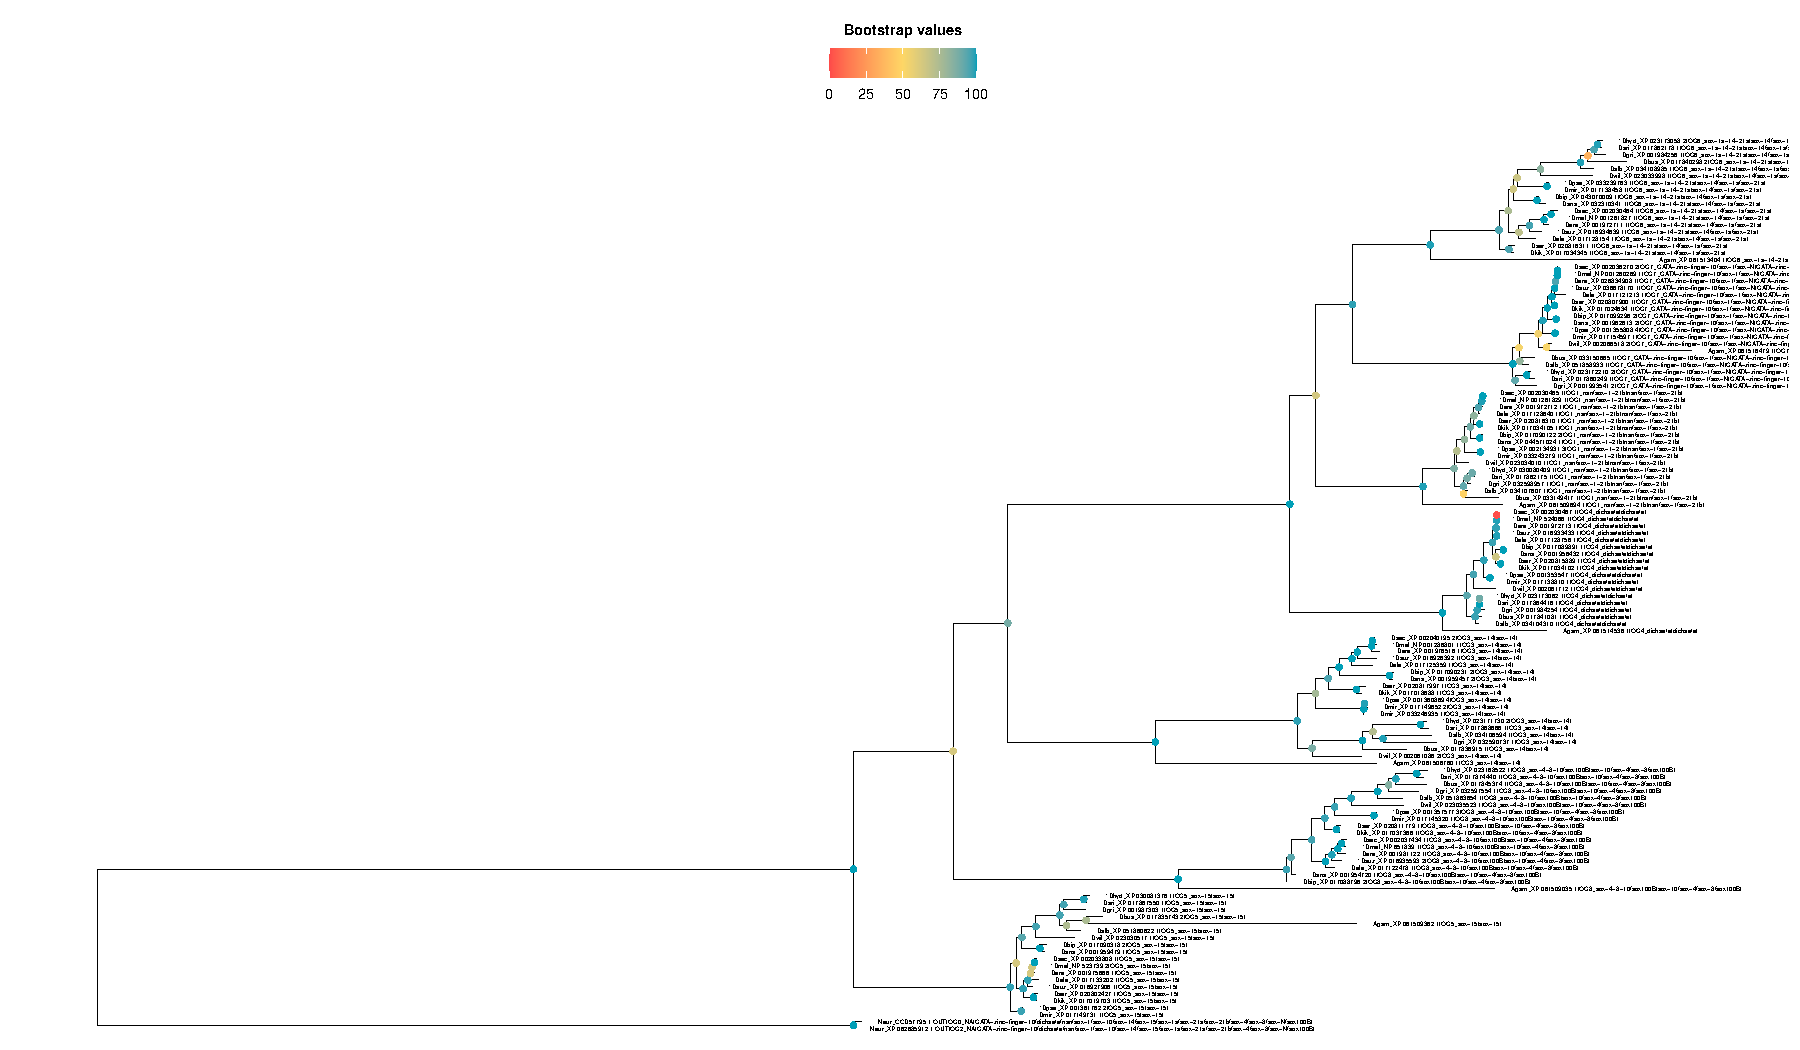
\includegraphics[width=\textwidth]{supp_figures/supp_fig_S9.pdf}
	\caption[\textbf{\gls{ml} phylogenetic tree of the \gls{sox} gene family in fruit flies, including the Possvm orthology inference}]
	{
		\textbf{\gls{ml} phylogenetic tree of the \gls{sox} gene family in fruit flies, including the Possvm orthology inference}. Reference genes from \gls{dmel}, \gls{dhyd}, \gls{dpse}, and \gls{dsuz} are marked with an asterisk at the beginning of the tip names. Species ID can be found in \cref{suppTab:drosophila_dataset}. Bootstrap values are shown for each node.
	}
	\label{suppFig:sox_drosophila}
\end{figure}

\begin{figure}[ht]
	\centering
	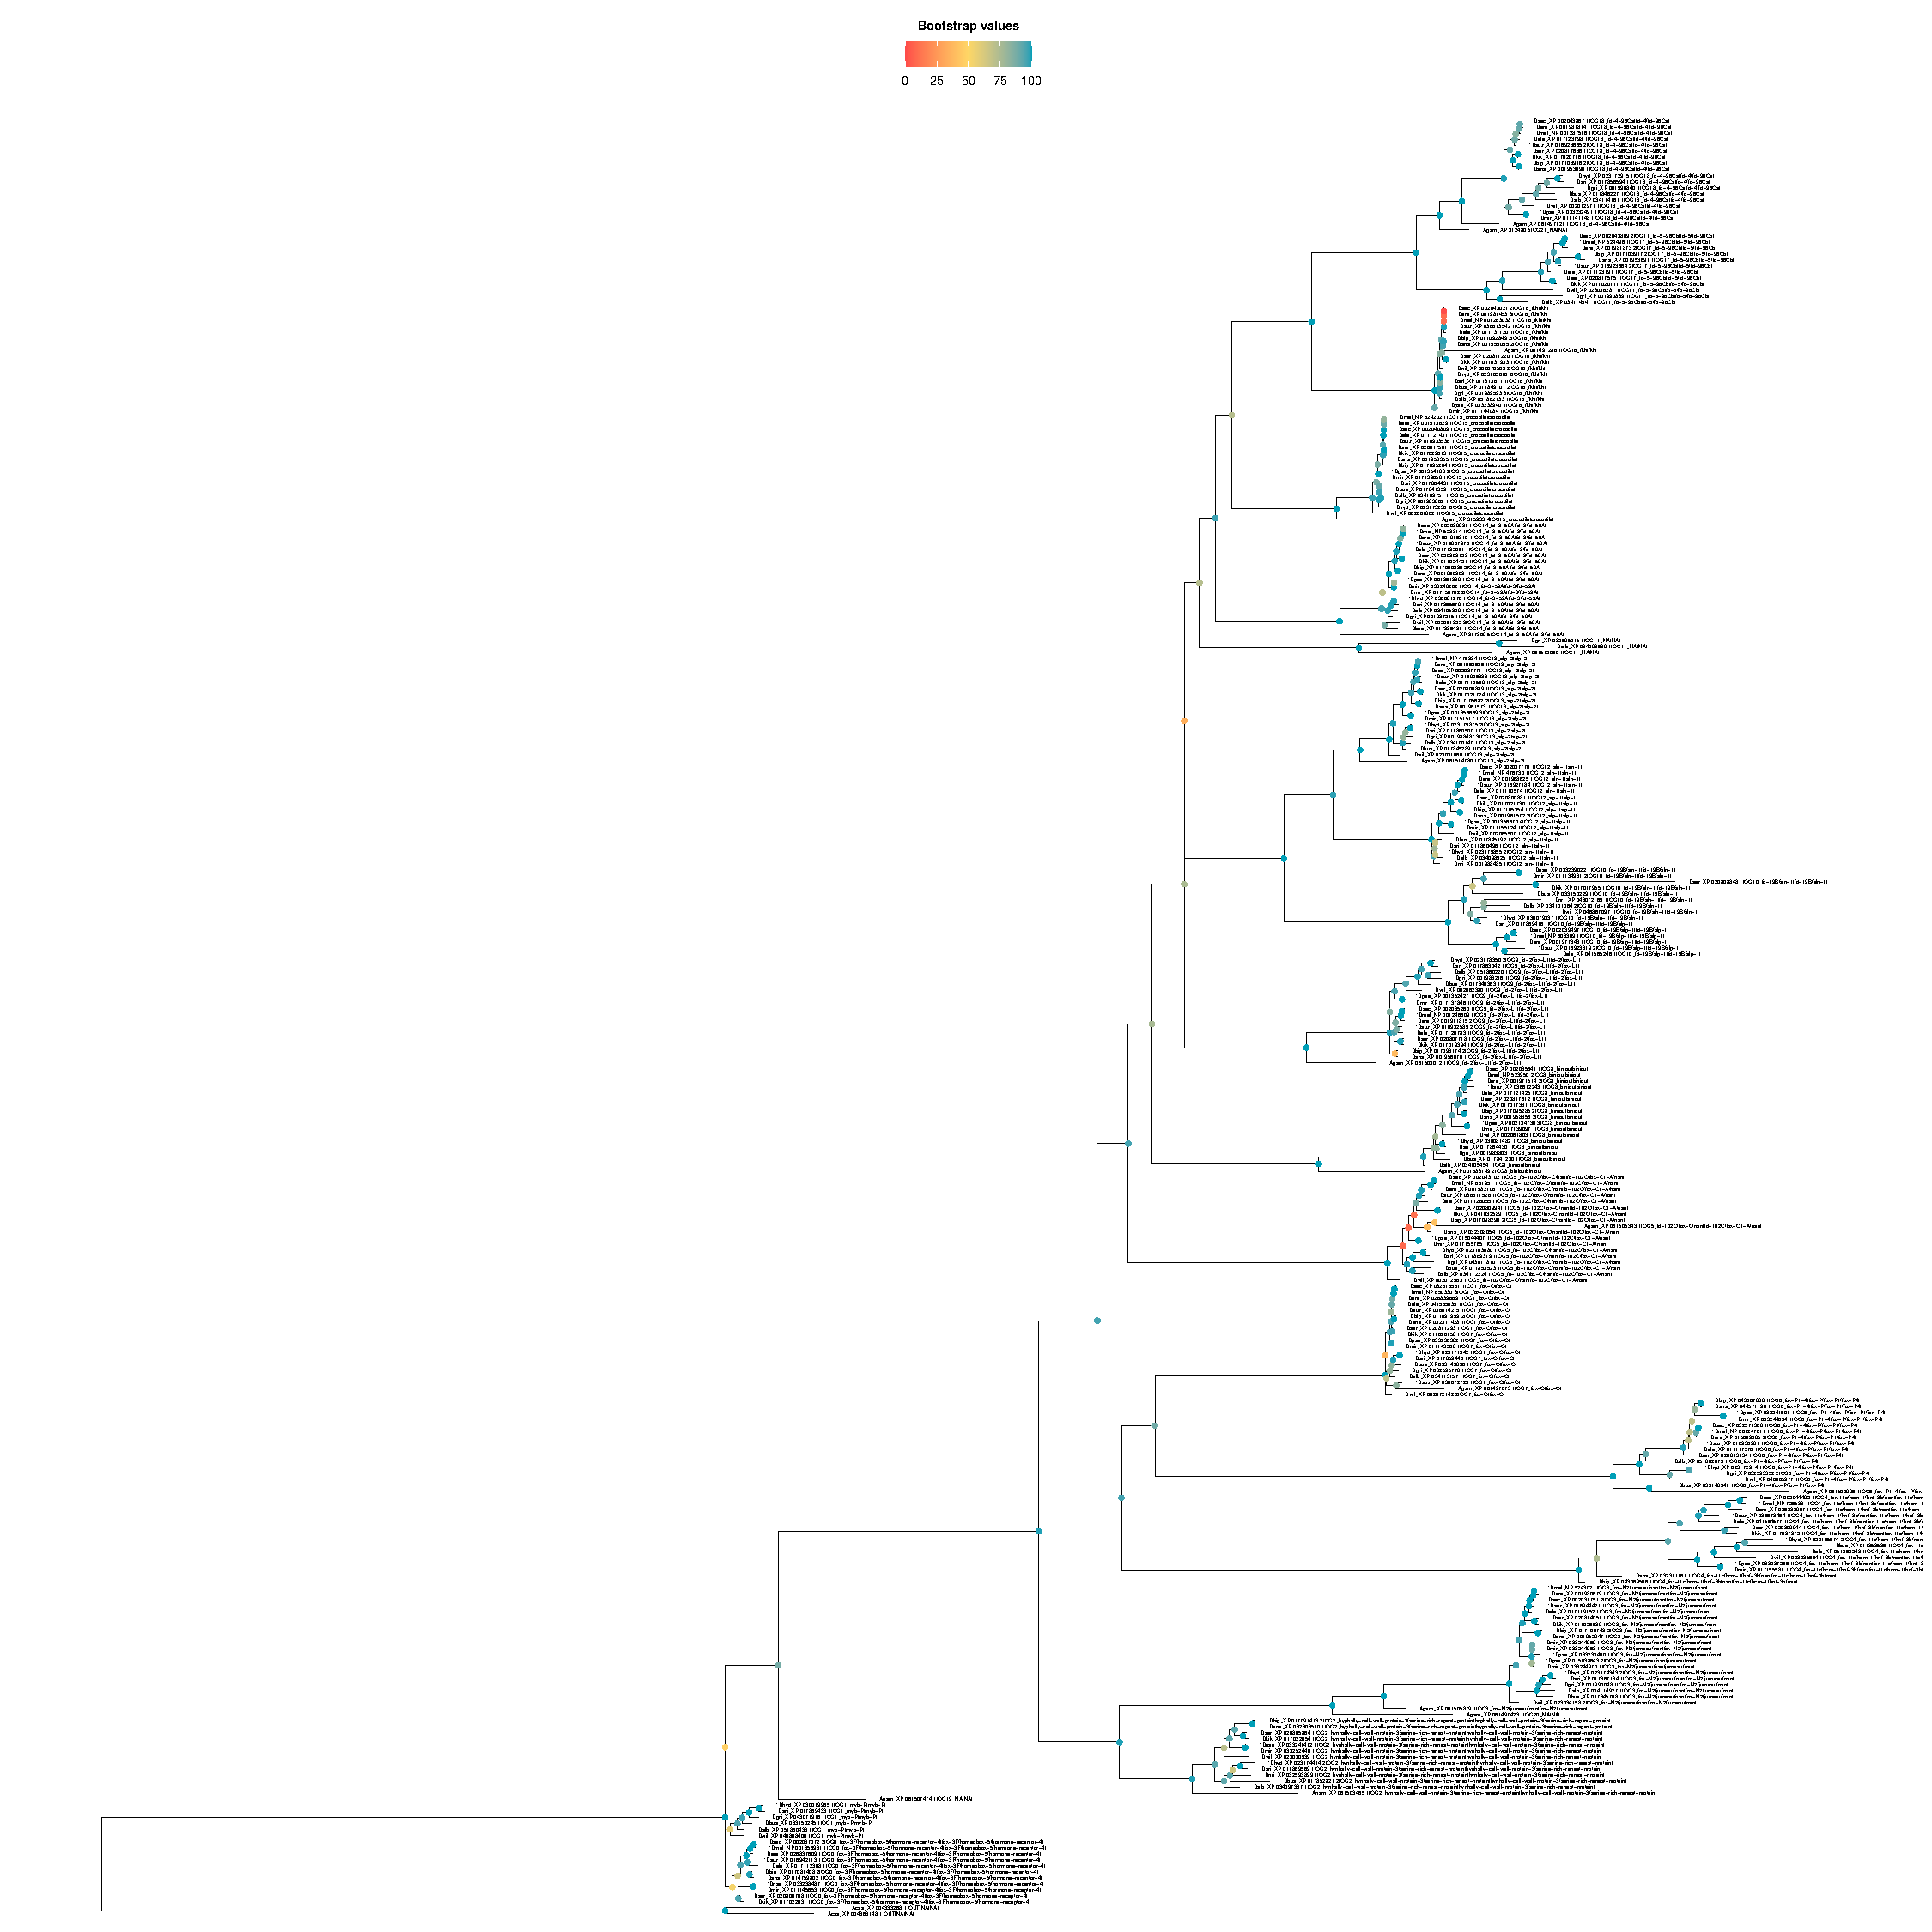
\includegraphics[width=\textwidth]{supp_figures/supp_fig_S10.pdf}
	\caption[\textbf{\gls{ml} phylogenetic tree of the \gls{fox} gene family in fruit flies, including the Possvm orthology inference}.]
	{
		\textbf{\gls{ml} phylogenetic tree of the \gls{fox} gene family in fruit flies, including the Possvm orthology inference}. Reference genes from \gls{dmel}, \gls{dhyd}, \gls{dpse}, and \gls{dsuz} are marked with an asterisk at the beginning of the tip names. Species ID can be found in \cref{suppTab:drosophila_dataset}. Bootstrap values are shown for each node.
	}
	\label{suppFig:fox_drosophila}
\end{figure}

\begin{figure}[ht]
	\centering
	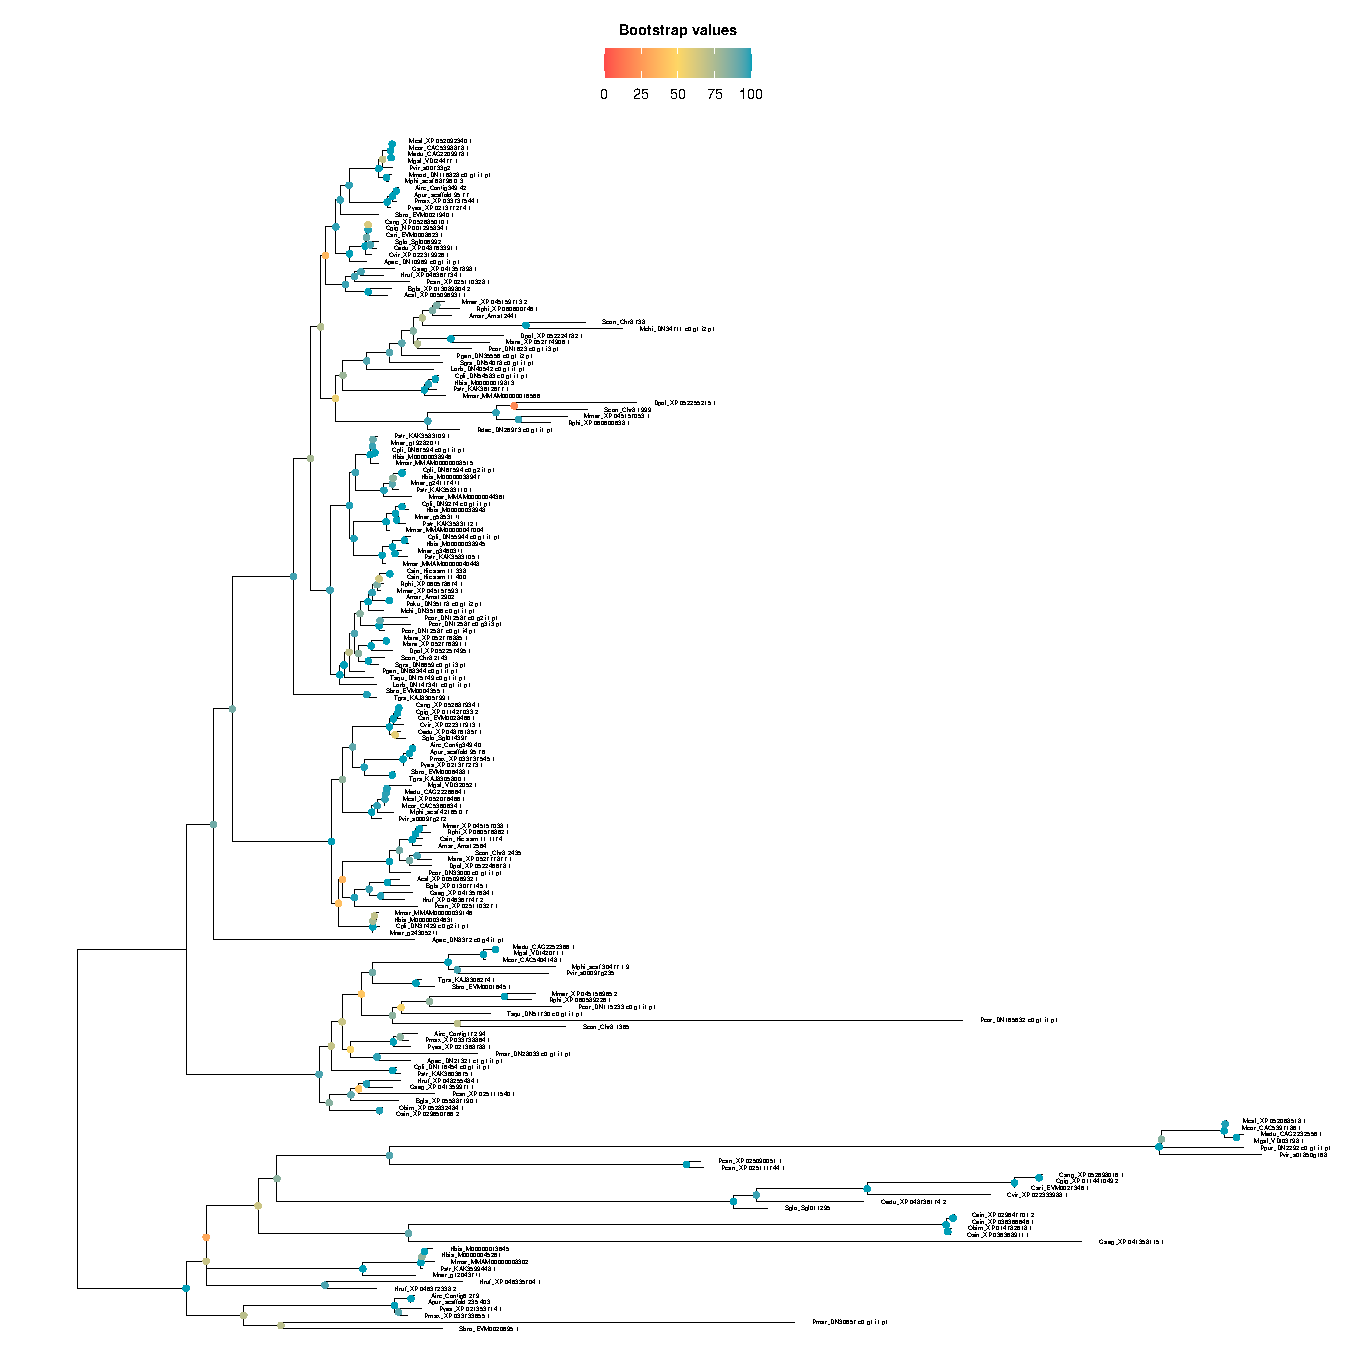
\includegraphics[width=\textwidth]{supp_figures/supp_fig_S11.pdf}
	\caption[\textbf{\gls{ml} phylogenetic tree of the \gls{dmrt} gene family in mollusc species}]
	{
		\textbf{\gls{ml} phylogenetic tree of the \gls{dmrt} gene family in mollusc species}. Species ID can be found in \cref{suppTab:bivalve_dataset}. The tree has been midpoint rooted. Bootstrap values are shown for each node.
	}
	\label{suppFig:dmrt_molluscOnly}
\end{figure}

\begin{figure}[ht]
	\centering
	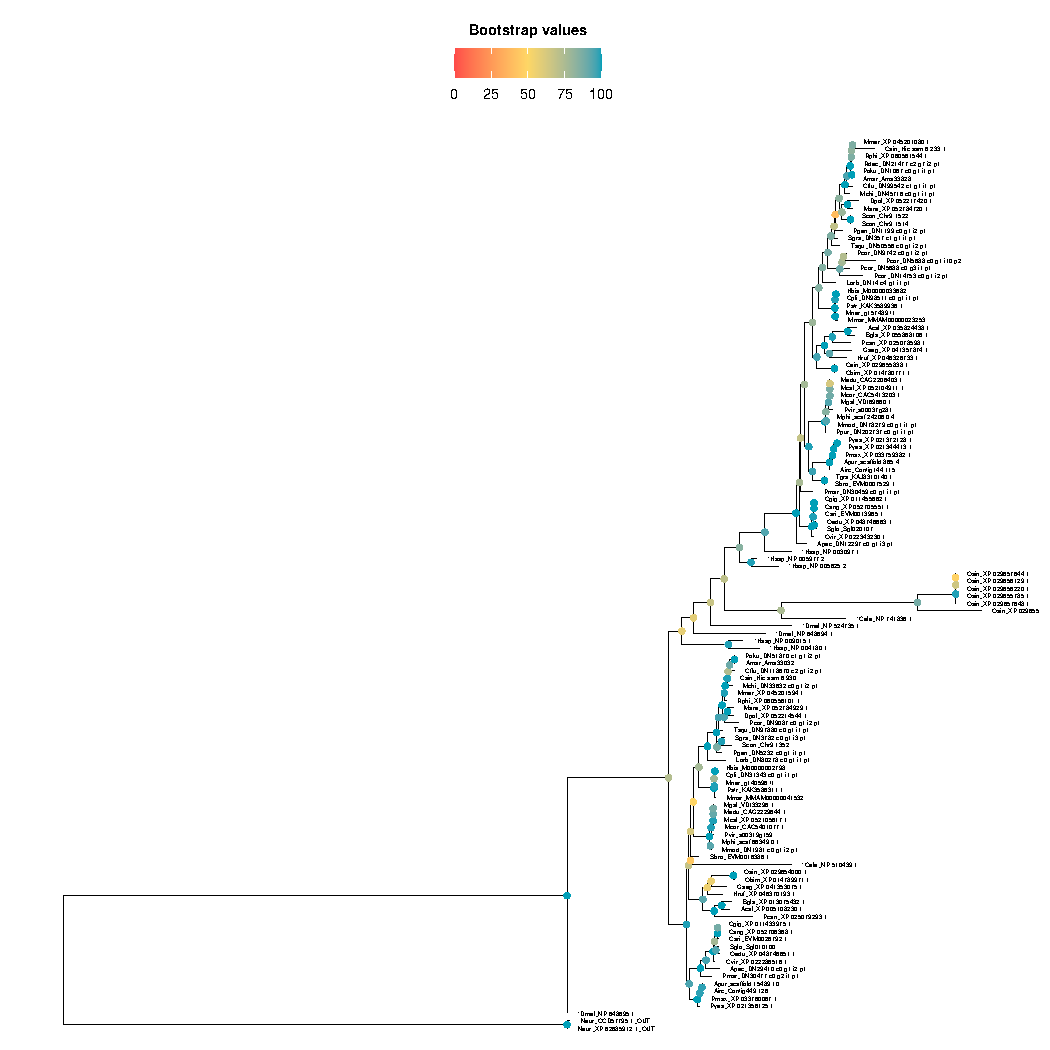
\includegraphics[width=\textwidth]{supp_figures/supp_fig_S12.pdf}
	\caption[\textbf{\gls{ml} phylogenetic tree of \textit{Sox-B1} and \textit{Sox-B2} genes in mollusc and reference species}]
	{
		\textbf{\gls{ml} phylogenetic tree of \textit{Sox-B1} and \textit{Sox-B2} genes in mollusc and reference species}. Reference genes from \gls{hsap}, \gls{cele}, and \gls{dmel} are marked with an asterisk at the beginning of the tip names. Species ID can be found in \cref{suppTab:bivalve_dataset}. Bootstrap values are shown for each node.
	}
	\label{suppFig:sox_B12}
\end{figure}

\begin{figure}[ht]
	\centering
	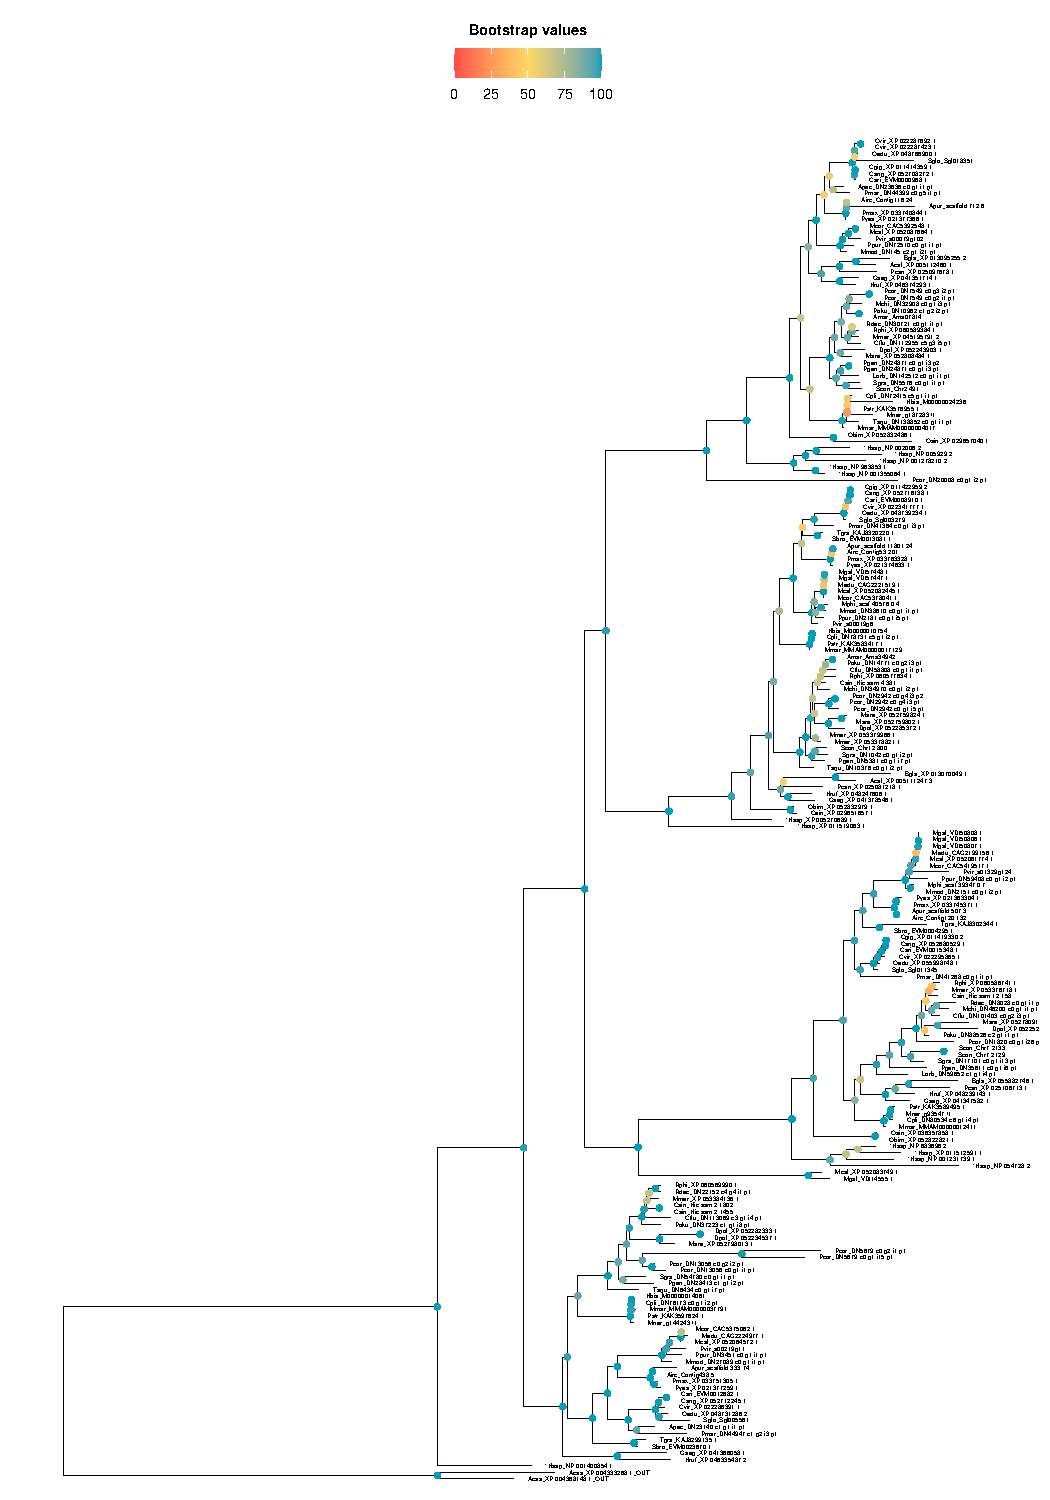
\includegraphics[height=0.85\textheight]{supp_figures/supp_fig_S13.pdf}
	\caption[\textbf{ML phylogenetic tree of \textit{Fox-J2}, \textit{Fox-M}, \textit{Fox-O}, and \textit{Fox-P} genes in mollusc and reference species}]
	{
		\textbf{ML phylogenetic tree of \textit{Fox-J2}, \textit{Fox-M}, \textit{Fox-O}, and \textit{Fox-P} genes in mollusc and reference species}. Reference genes from \textit{H. sapiens}, \textit{C. elegans}, and \textit{D. melanogaster} are marked with an asterisk at the beginning of the tip names. Species ID can be found in \cref{suppTab:bivalve_dataset}. Bootstrap values are shown for each node.
	}
	\label{suppFig:fox_JMOP}
\end{figure}

\begin{figure}[ht]
	\centering
	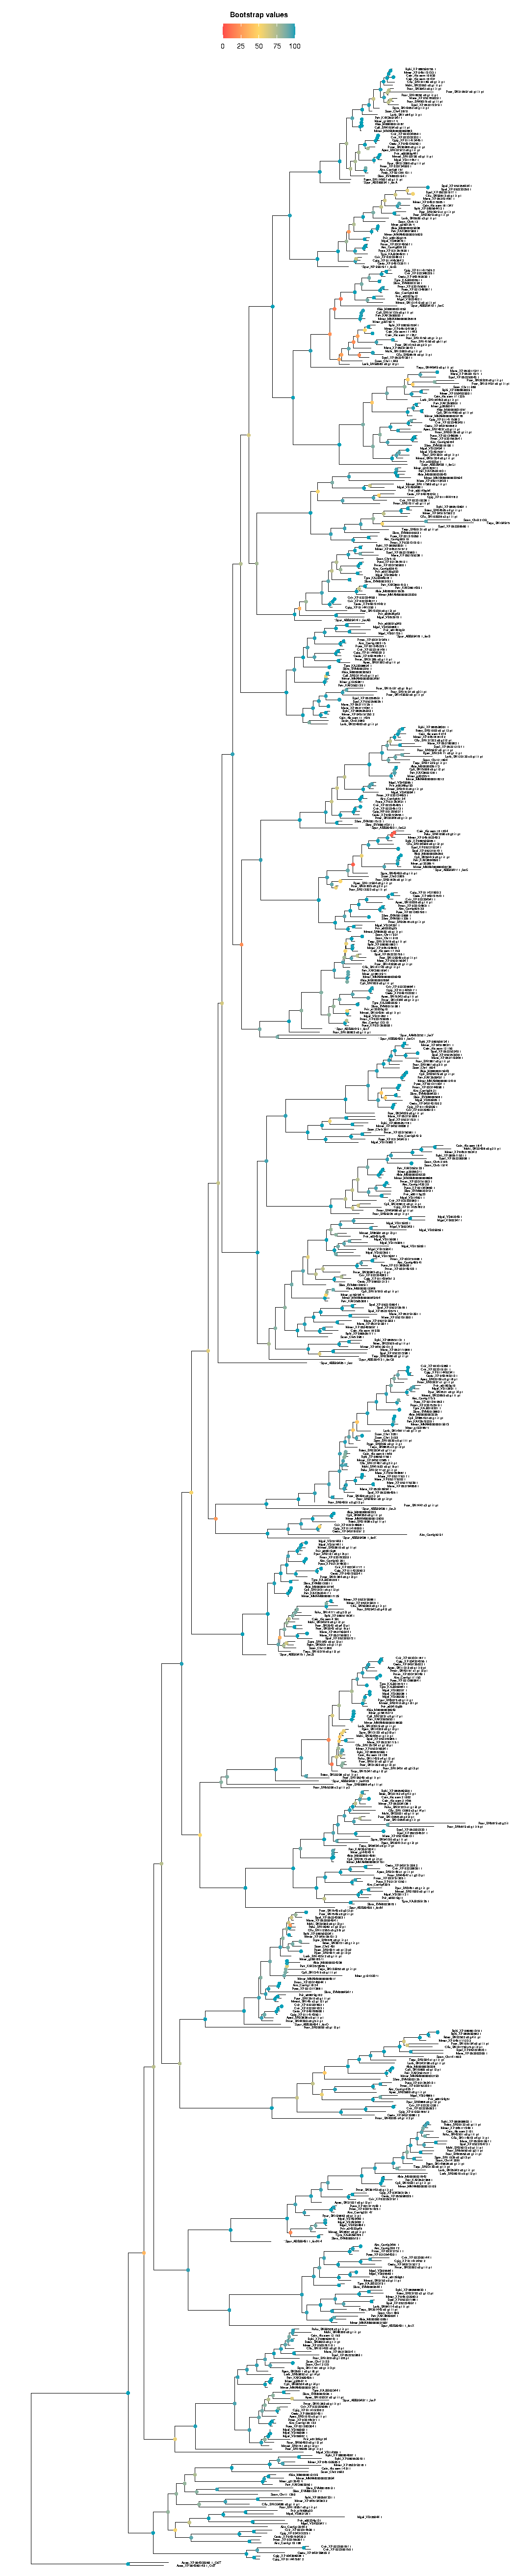
\includegraphics[height=0.85\textheight]{supp_figures/supp_fig_S14.pdf}
	\caption[\textbf{\gls{ml} phylogenetic tree of the Fox gene family in bivalves and the sea urchin \gls{spur} (Spur)}]
	{
		\textbf{\gls{ml} phylogenetic tree of the Fox gene family in bivalves and the sea urchin \gls{spur} (Spur)}. Reference genes from \gls{spur} are marked with an asterisk at the beginning of the tip names. Species ID can be found in \cref{suppTab:bivalve_dataset}. \gls{spur} genes are those given by \citebold{tu2006sea}. Bootstrap values are shown for each node.
	}
	\label{suppFig:fox_spur}
\end{figure}

\begin{figure}[ht]
	\centering
	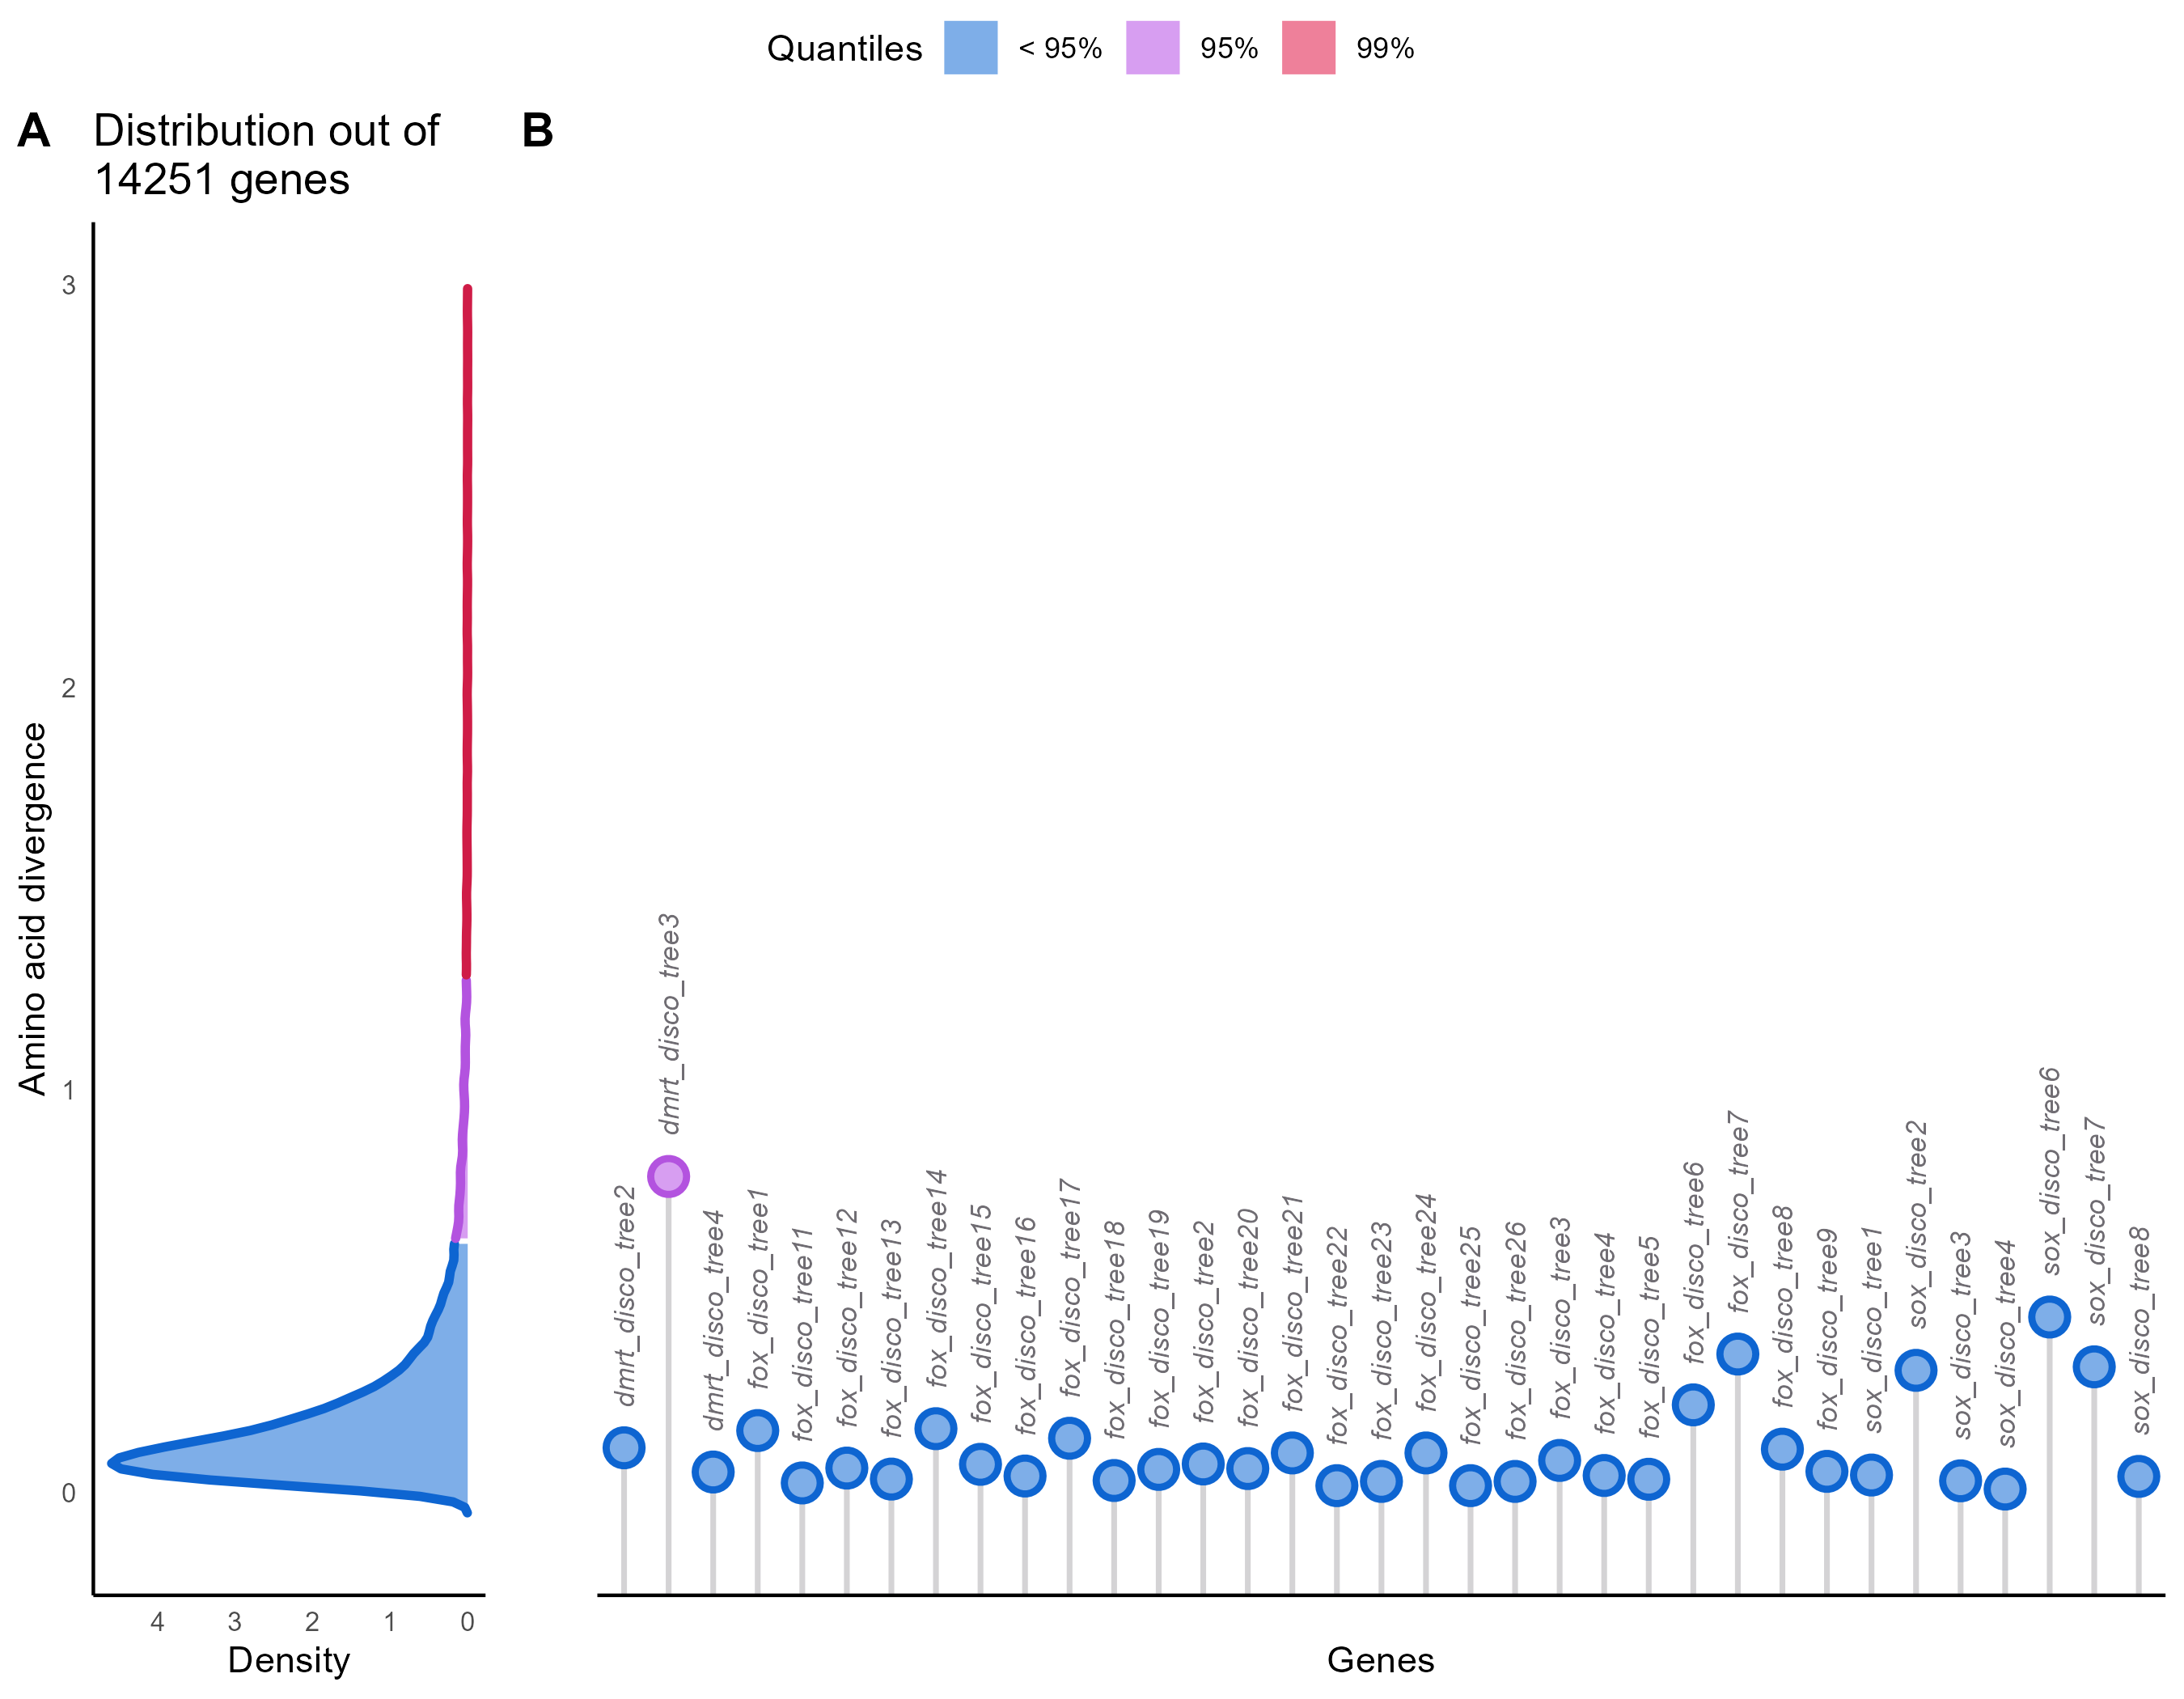
\includegraphics[width=\textwidth]{supp_figures/supp_fig_S15.png}
	\caption[\textbf{Distribution of \gls{aasd} of single-copy orthogroups in \gls{cgig}, \gls{cang}, \gls{cari}, and \gls{cvir} (A), including \gls{dsfg} (B)}]
	{
		\textbf{Distribution of \gls{aasd} of single-copy orthogroups in \gls{cgig}, \gls{cang}, \gls{cari}, and \gls{cvir} (A), including \gls{dsfg} (B)}. The distribution of \gls{aasd} in \textit{Crassostrea} has been computed on the median values of pairwise distances of over \qty{14}{\kilo\nothing} \glspl{sco}. Circle heights of \glspl{dsfg} show the median value of their \gls{aasd}. \textit{Dmrt-1L} genes are indicated as ‘dmrt\_disco\_tree3’.
	}
	\label{suppFig:DSFG_crassostreaDivergence}
\end{figure}

\begin{figure}[ht!]
	\centering
	\includegraphics[width=0.9\textwidth]{supp_figures/supp_fig_S16.png}
	\caption[\textbf{MitoTracker staining and negative controls of mRNA \textit{in-situ} \gls{hcr} in in \gls{mgal} (A) oocyte, (B) 2-cell male embryo, (C) 4-cell female embryo, (D) 8-cell female embryo, (E) \qty{12}{\hpf} embryo (gastrula), and (F) \qty{48}{\hpf} larvae (D-veliger)}]
	{
		\textbf{MitoTracker staining and negative controls of mRNA \textit{in-situ} \gls{hcr} in \gls{mgal} (A) oocyte, (B) 2-cell male embryo, (C) 4-cell female embryo, (D) 8-cell female embryo, (E) \qty{12}{\hpf} embryo (gastrula), and (F) \qty{48}{\hpf} larvae (D-veliger)}. Nuclei are shown in white; in the 2-, 4-, and 8-cell stages, nuclei are also marked with numbers; in the 8-cell stage, nuclei of blastomeres in the background are highlighted with dashed circles. Sperm mitochondria, when stained (shown in green), are marked with arrowheads. Acquisition channels are indicated on top, and colours are the same as in \cref{fig:hcr}. h: hinge; nu: oocyte nucleus. Scale bar: \qty{20}{\um}.
	}
	\label{suppFig:hcrBianco}
\end{figure}

\begin{figure}[ht!]
	\floatbox[{\capbeside\thisfloatsetup{capbesideposition={right,top},capbesidewidth=0.4\textwidth}}]{figure}[\FBwidth]
	{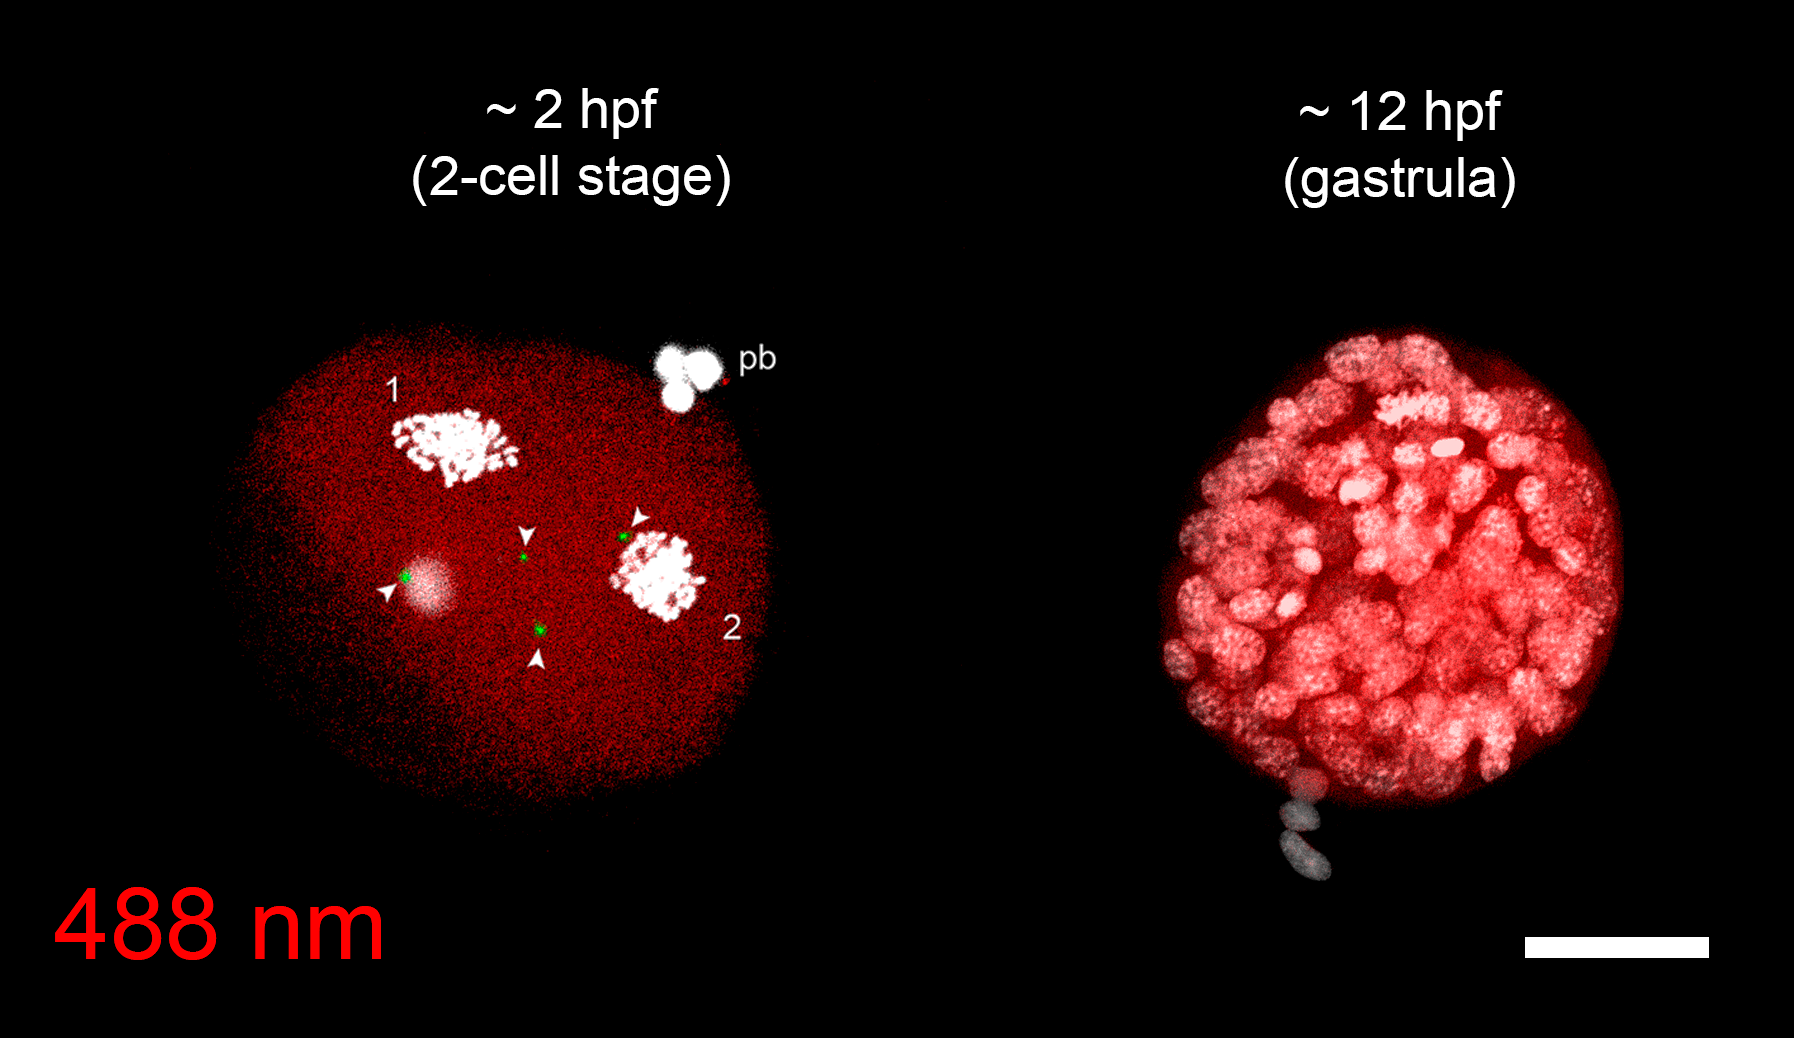
\includegraphics[width=0.5\textwidth]{supp_figures/supp_fig_S17.png}}
	{\caption[\textbf{MitoTracker staining and negative controls of Vasa immunolocalization in \gls{mgal} embryos}]
	{
		\textbf{MitoTracker staining and negative controls of Vasa immunolocalization in \gls{mgal} embryos}. Nuclei are shown in white. Sperm mitochondria (in green) are marked with arrowheads. pb: polar body. Scale bar: \qty{20}{\um}.
	}
	\label{suppFig:immunoBianco}}
\end{figure}

\clearpage

% \end{document}